\documentclass[10pt,letterpaper]{article}

\usepackage{cogsci}
\usepackage{pslatex}
\usepackage{amsmath}
\usepackage{amsfonts}
\usepackage{apacite}
\usepackage{graphicx}
\usepackage{caption}
\usepackage{subcaption}
\usepackage{etex}
\usepackage{tikz}

\title{The Funny Thing About Incongruity: A Noisy Channel Model of Puns}
 
\author{{\large \bf Justine Kao (justinek@stanford.edu)} \\
  Department of Psychology \\
  Stanford, USA
  \AND {\large \bf Noah Goodman (ngoodman@stanford.edu)} \\
  Department of Psychology \\
  Stanford, USA
   \AND {\large \bf Roger Levy (rlevy@ucsd.edu)} \\
  Department of Linguistics \\
  UCSD, USA
  }


\begin{document}

\maketitle

\begin{abstract}

``Researchers showed the robot ten puns, hoping that one of them would make it laugh. Unfortunately, no pun in ten did."

\textbf{Keywords:} 
Humor; language understanding; noisy channel; probabilistic models; sentence processing
\end{abstract}
\section{Introduction}
Humor plays an essential role in human interactions. In a study on gender differences in desired characteristics of relationship partners, both men and women rated sense of humor as one of the most important qualities, above physical attractiveness and earning potential \cite{stewart2000sex}. Humor has important positive effects on children's development \cite{frank1989humor}, success in the work place \cite{duncan1990humor}, marital satisfaction \cite{ziv1989humor}, and coping with illness and traumatic events \cite{johnson2002use, gelkopf1996humor}. In this paper, we are interested in understanding how this fundamental and ubiquitous phenomenon works from the perspective of cognitive science. What makes something funny? How might the defining characteristics of humor shed light on the ways in which the mind processes and evaluates information?
\subsection{Incongruity theory of humor}
A leading theory in humor research is that incongruity is a necessary condition for humor \cite{veale2004incongruity, forabosco1992cognitive, mcghee1979humor, martin2007psychology, hurley2011inside}. As Veale (2004) states, ``Of the few sweeping generalizations one can make about humor that are neither controversial or trivially false, one is surely that humor is a phenomenon that relies on incongruity." Although there is disagreement in the literature about whether incongruity alone is sufficient, most theorists accept that humor requires perceiving a situation from different viewpoints and finding the subsequent interpretations of the same situation to be incompatible \cite{veatch1998theory, forabosco1992cognitive}. 

Take for example the sentence: ``I dropped out of Communism class because of lousy Marx." There is a strong intuition upon ``getting" the joke that two distinct and globally coherent interpretations are present. Either the protagonist dropped out of Communism class because she had negative feelings about Karl Marx, or because she received bad grades. Since the interpretations represent two different situations, humor theorists would describe them as being incongruous and thus funny. However, humor theorists' definitions of incongruity are often ambiguous and leave room for interpretation, making it difficult to test the role of incongruity empirically \cite{veale2004incongruity}. 

In this paper, we propose a computational model of humor that formalizes the concept of incongruity. Since humor is a complex phenomenon that relies heavily on background knowledge and discourse understanding beyond the scope of this paper, we focus on applying formalizations of incongruity to a subset of linguistic humor: puns. In particular, we test the role of incongruity in producing humorous sensations in phonetically ambiguous sentences. 

\subsection{Computational humor}
Given the prevalence of humor in human communication, researchers in artificial intelligence have argued that computers should be able to generate and detect humor in order to interact with humans more naturally and effectively \cite{mihalcea2006learning}. As a result, computational humor has made important progress and also received attention from popular press in the last decade (insert NYT citation here). However, most of the work in computational humor has focused either on utilizing joke-specific templates and schemata \cite{binsted1996machine, kiddon2011s}, or identifying linguistic features such as slang and alliteration that strongly predict humorous intent \cite{mihalcea2006learning, semantic2010}. The former type of studies is restricted to identifying jokes with a very specific format and structure, while the latter type falls short of testing or building upon deeper and more general theories of humor involving the management of incongruity. 

Our work moves beyond these two types of approaches and directly utilizes incongruence to identify humorous texts. Given that humor theorists view incongruity as an essential component of jokes, we examine whether human judgments of funniness can be predicted by the presence of incongruous interpretations of the same input. In particular, we aim to develop a formal model of linguistic humor that fits naturally into the framework of normal language processing. We propose that a noisy channel approach to language processing allows the comprehender to consider alternative viewpoints and interpretations of the same linguistic input and can account for the possibility of incongruity. 

Our purposes for developing a formal model of linguistic humor are thus two-fold. First, we wish to formalize the concept of incongruity and test assumptions adopted by leading theories in humor research. Secondly, we aim to show that a noisy channel of language comprehension allows for the flexibility in context selection and interpretation that gives rise to sophisticated linguistic and social meaning such as humor. 

\section{The Noisy Channel and Incongruity}
A central assumption in noisy channel models of sentence comprehension is that comprehenders maintain uncertainty about the linguistic input and consider close alternatives during processing in order to arrive at a globally coherent interpretation \cite{levy2008noisy, levy2009eye}. Previous work on noisy channel models of sentence comprehension has shown that such models are able to explain interpretation patterns of sentences with verb omission errors \cite{bergenverb}, garden path sentences \cite{levy2011integrating}, and word order variation across languages \cite{gibsonnoisy}. These studies validate the idea that language comprehension is a rational process that incorporates uncertainty at the level of word-level input to affect sentence-level comprehension \cite{levy2009eye}.

Given that sentence comprehension involves uncertainty about the linguistic input, when the comprehender detects incoherence at the sentence level, alternatives are considered. This process allows the comprehender to maintain multiple interpretations at the word level that may each be globally coherent but incongruous with each other. The notion of incongruity thus fits naturally into a noisy channel model of sentence comprehension and can be formalized as such to explain its role in humor. 


%% cite semantic priming

\subsection{Homophone puns: a hare-y issue}
In this paper, we restrict the scope of our model to homophone puns---puns where ambiguity arises from the presence of a phonetically ambiguous word---for two reasons. First, homophone puns have a relatively clearly defined and constrained space of possible interpretations. Since distinct interpretations of the sentence hinge on one phonetically ambiguous word, interpretations at the sentence level are relatively shallow and can be approximated by the two lexical forms of the homophone word. An example helps illustrate this idea: 
\begin{itemize}
\item [] \emph{``The magician got so mad he pulled his hare out."} 
\end{itemize}
There are two interpretations of this sentence:
\begin{itemize}
\item[(a)] The magician got so mad he (idiomatically) pulled out the hair on his head.
\item[(b)] The magician got so mad he performed the trick of pulling a rabbit out of his hat.
\end{itemize}

The difference between interpretations (a) and (b) can be approximated by the two interpretations of the word ``hare." Either the comprehender interprets ``hare" as its close alternative (``hair"), leading to interpretation (a), or as itself (``hare"), leading to interpretation (b). Thus, homophone puns allows us to approximate differences in sentence-level interpretations as differences in word-level interpretations.
 
Another reason to focus on homophone puns is that they reflect the role of semantic information in lexical disambiguation. Importantly, ambiguity alone is not enough for humor; plenty of sentences contain phonetically ambiguous words and yet are not funny. For example, \emph{``The professor got so mad he pulled his hair out}" is not a pun, just an unfortunate situation. The detection of a pun relies on successful identification of contextual cues within a sentence or discourse that support different interpretations and boost the likelihoods of different interpretations (e.g. ``pulled" supports the interpretation of``hair"; ``magician" supports the interpretation of ``hare."). Previous research suggests that efficient lexical processing involves automatic semantic association with neighboring words \cite{seidenberg1982automatic}. Other work has shown the effects of lexical priming on processing sentences with lexical ambiguity \cite{simpson1981meaning, burke1984semantic, smith2011cloze}. Given the difficulties of directly computing the probability of an interpretation given a context, we leverage lexical association to compute the interpretation probabilities of a phonetically ambiguous word.

Writer and philosopher Henri Bergson defined a pun as ``a sentence or utterance in which two ideas are expressed, and we are confronted with only one series of words." We propose that the reason why two ideas can be communicated through only one set of words is because comprehenders maintain uncertainty about the input and consider alternative meanings distinct from what is directly observed. For example, if a comprehender does not maintain uncertainty about the observed word ``hare," the alternative meaning ``hair" would never be considered regardless of the contextual cues that are presented in the sentence.

Based on this intuition, our model adopts a noisy channel approach that allows for multiple interpretations of an ambiguous item. Under the assumption that lexical priming plays a role in disambiguation during sentence processing, semantic associations with each of the surrounding words are used to compute the probabilities of each candidate interpretation. Motivated by the incongruity theory of humor, we predict that a sentence in which the meaning distribution for the ambiguous word is bimodal (i.e. has two similarly likely interpretations in context) is more likely to be funny. We present our model more formally in the following section.

\section{Model}

Suppose a sentence $S$ is composed of words $w = \{w_1, \dots ,w_n\}$ and $h$. $h$ is a phonetically ambiguous word that has two homophone interpretations or meanings, $m_1$ and $m_2$. 

We propose a generative model of the sentence in which the latent varialbe $m$ generates the observed words $w$ and $h$. We introduce an indicator variable $f$ in the model that determines whether each word in a sentence is ``in semantic focus;" in other words, whether it was generated due to semantic relevance to the $m$ or to chance. This allows the model to consider alternative subsets of the sentence as the primary context. (I'm not sure if I'm describing reasons for  $f$ very convincingly...) %%

With some probability $P(f)$, a word $w$ is in focus and generated due to semantic relevance to $m$. If this is the case, the word $w$ is drawn from the distribution $P(w | m)$. Otherwise, $w$ is drawn from an alternative distribution $P(w | m')$, where $m'$ is a homophone of $m$. With some probability, $h$ is the lexical form of the latent meaning variable $m$; otherwise, $h$ was corrupted during production and is the lexical form of $m'$.

\begin{center}
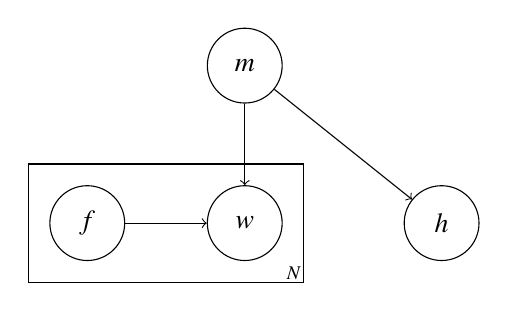
\begin{tikzpicture}
\tikzstyle{place}=[circle,draw,inner sep=2pt,minimum size=0.95cm]
 \tikzstyle{plate}=[rectangle,draw,inner sep=0pt]
 \node[place] (m) at (-5,3) {$m$};
 \node[place] (w) at (-5,1) {$w$};
 \node[place] (h) at (-2.5, 1) {$h$};
  \node[place] (f) at (-7, 1) {$f$};
 %\node[place] (wordsprior) at (0,4.5) {$\wordsprior$};
 \draw [->] (m) -- (w);
 \draw [->] (m) -- (h);
  \draw [->] (f) -- (w);
 
 %\draw [->] (wordsprior) -- (phi);
 \node[plate, minimum height=1.5cm, minimum width=3.5cm] (plateC1n) at (-6,1) {};
 \node at (plateC1n.south east) [above left, inner sep=.1em] {\scriptsize $N$};

\end{tikzpicture}
\end{center}

Given our generative model and the observed words $w$ and $h$, we can infer the probability distribution of the latent variable $m$. We then compute a measure of the distribution $P(m)$ that quantifies its degree of incongruity (can be more clearly described...) %%

There are three steps to arrive at a measure of incongruity: (1) compute the probability of a set of words being in semantic focus (2) given the set of context words $C$ being in focus, compute the distribution $P(m | C)$ (3) Marginalize out selections of words in focus to arrive at $P(m)$ and compute the incongruity of $P(m)$. Since the probability of a set of words $C$ being in focus is simply $P(f)^{|C|}$, we focus on describing parts (2) and (3) in more depth.

\subsection{Computing interpretation probabilities}
Suppose a context $C = \{c_{1}, \dots, c_{k}\}$ is in focus. Since $h$ itself (the phonetically ambiguous word) can also be in $C$, we treat it as the same as any other word $c$ in focus and omit it for the simplicity of notation. 

Since $C$ is in semantic focus, from our generative model, $C$ was generated independently given $m$. To compute the probability distribution of $m$ given $C$, by Bayes' Theorem, 
$$
P(m | c_1, \dots, c_k)  = P(m) \frac{P(c_1,\dots, c_k | m)}{P(c_1,\dots, c_k)}
$$
Our generative model already assumes conditional independence of $C$ on $m$. We further make the approximation that words in $C$ are independent as well. Thus,
$$
P(m | c_1, \dots, c_k) = P(m) \prod_1^k \frac{P(c_i | m)}{P(c_i)} 
$$
\subsection{Computing incongruity}
%%
*Major revision pending model adjustments

Given the derivations above, we compute the interpretation probabilities of $h$ for any two contexts $C_1$ and $C_2$.

We can thus compute the interpretation distributions of $m$ given $C_1$ and $C_2$, denoted as the following: $C_1(m)$ and $C_2(m)$. Since $C_1(m)$ and $C_2(m)$ are two probability distributions, we can compute their distance using standard measures from information theory. Since incongruity between two contexts should be symmetric, we select symmetrised KL divergence, defined as the following:
$$
D_{KL}(P || Q) + D_{KL}(Q || P) = \sum_x \bigg ( \ln \frac{P(x)}{Q(x)} P(x) +  \ln \frac{Q(x)}{P(x)} Q(x) \bigg )
$$
Given two contexts $C_1$ and $C_2$, the distance in meaning distributions of $h$ is given by the following:
$$
\sum_i \bigg ( \ln \frac{P(m_i | C_1)}{P(m_i | C_2)} P(m_i | C_1) +  \ln \frac{P(m_i | C_2)}{P(m_i | C_1)} P(m_i | C_2) \bigg )
$$
Summing over all context combinations, our measure of a sentence's incongruity is the sum of the symmetrised KL distance for each context combination weighted by the probability of selecting those contexts:
$$
 \sum_{C_1, C_2} P(C_1) P(C_2) \sum_i \bigg ( \ln \frac{P(m_i | C_1)}{P(m_i | C_2)} P(m_i | C_1) +  \ln \frac{P(m_i | C_2)}{P(m_i | C_1)} P(m_i | C_2) \bigg )
$$
Under this framework, $m_i$ can be any existing meaning. However, for simplicity, we assume that given the written word $h$ in $C_1$ and $C_2$, $P(m_k | C_1) = P(m_k | C_2) = \epsilon$ for all $m_k$ that are not exact homophones of $h$ and can be ignored. Thus we are only interested in interpretations $m_1$ and $m_2$, which are exact homophones of the written word $h$.

By combining a noisy channel model of language processing, a Bayesian model for meaning distributions, and a standard information theoretic measure of symmetrised KL divergence, our model presents a formal measure of incongruity to test the incongruity theory of humor.  

\section{Evaluation}
We evaluate our model on a set of $160$ sentences, consisting of $40$ puns, $80$ control non-pun sentences that match the puns in containing the same phonetically ambiguous words, and $40$ ``de-punned" control sentences that are matched with a subset of the puns but with certain manipulations described below. We evaluate our model based on how well it predicts people's funniness ratings of these sentences.
\subsection{Materials}
We selected $40$ pun sentences from a large collection of puns on a website called �Pun of the Day,� which contains over a thousand original puns. Puns were selected such that the ambiguous item is a single phonetically ambiguous word, and such that no two puns in the collection have the same ambiguous item. 

The $80$ non-pun sentences were chosen to match each pun sentence on its ambiguous word as well as the alternative homophone. The sentences were taken from an online version of Heinle's Newbury House Dictionary of American English (http://nhd.heinle.com/). We selected sample sentences included in the definition of the homophone word. This design ensured that puns and non-pun sentences contain the same phonetically ambiguous words, a control that was not used in previous work on automatic humor recognition.

We also constructed $40$ sentences to be minimally different from the pun sentences, which we will call de-punned sentences. A research assistant who was blind to the hypothesis and model was asked to replace one word in each of the pun sentences (without changing the homophone word itself) so that the sentence is still sensible but is no longer a pun. This resulted in sentences that were only one word different from the pun sentences. Below are example sentences from each category.\\\\
\begin{tabular}{| l | l |}\hline
\textbf{Type} & \textbf{Example} \\\hline
Pun & ``The magician got so mad he pulled his hare out." \\
De-pun & ``The teacher got so mad he pulled his hare out."\\
Normal & ``The hare ran rapidly across the field."\\
Normal & ``Some people have lots of hair on their heads."\\\hline
\end{tabular}\\\\

\subsection{Human ratings of semantic relatedness}

\begin{figure}[t]
\scalebox{0.44}{\includegraphics{Plots/hare_pun.png}}
\caption{Relatedness of word pairs in example pun.}
\end{figure}

\begin{figure}[t]
\scalebox{0.44}{\includegraphics{Plots/hare_nonpun.png}}
\caption{Relatedness of word pairs in example non pun.}
\end{figure}

As described in the model section, in order to compute interpretation probabilities of the homophone word given different contexts, we need the conditional probabilities of each word in the context given the homophone word, $P(c | m)$. However, $P(c | m)$ is difficult to obtain through corpora (due to data sparsity) as well as through empirical measures of association strength (due to the large number of subjects one must recruit in order to obtain a good estimation of subjects' likelihood of thinking of $c$ given $m$). We approximate $P(c | m)$ using empirical measures of the semantic relatedness between $c$ and $m$, denoted as $R(c, m)$. We use $R(c, m)$ as an approximate measure of point wise mutual information between $c$ and $m$, defined as follows:
$$
pmi(c, m)= {\log \frac{P(c, m)}{P(c)P(m)}} = \log \frac{P(c | m)}{P(c)} = \log P(c | m) - \log P(c)
$$
With the proper substitutions, the derivation of $P(m | c_1, \dots, c_l, h)$ in log space can be reduced to the following:
$$
\log P(m | c_1, \dots, c_k)
= \log P(m) + \sum_1^k \log P(c_i | m) - \sum_1^k \log P(c_i)} 
$$
$$
= \log P(m) + \sum_i^k R(c_k, m) 
$$

To obtain $R(c, m)$ for each of the words $c$ in the stimuli sentences, we recruited $200$ subjects on Amazon's Mechanical Turk to rate distinct word pairs on their semantic relatedness. Function words were removed from the sentences, and the remaining words were paired with each of the interpretations of the homophone sequence (e.g., ``magician" and ``hare" is a legitimate word pair, as well as ``magician" and ``hair"). This resulted in $1460$ distinct word pairs. Each subject saw $146$ pairs of words in random order and were asked to rate how related each word pair is from $1$ to $10$. The average split-half correlation of the relatedness ratings was $0.916$. 

Figure 1 and 2 show the relatedness of content words in the sentence with the two homophone interpretations. We see that in the pun sentence, the word ``magician" is rated as significantly more related to ``hare" than it is to ``hair", while the word ``pulled" is rated as significantly more related to ``hair" than it is to ``hare." On the other hand, all words in the non-pun example are significantly more related to the word ``hare" than to ``hair."

Figure 3 shows the average relatedness ratings of words and the two homophone interpretations across the three types of sentences. In pun sentences, the average relatedness of words to the two homophone interpretations are roughly equivalent. In the non-pun sentences, the average relatedness of words to the observed homophone is significantly higher than to the alternative homophone. This analysis of human ratings of relatedness supports the intuition on which our model is based that funnier sentences are those in which different contexts support incongruous interpretations of the homophone.



\begin{figure}[t]
\scalebox{0.45}{\includegraphics{Plots/ave_relatedness.png}}
\caption{Average relatedness ratings across sentence types}
\end{figure}

\subsection{Human Ratings of Funniness}
We obtained funniness ratings of the sentences from a separate pool of subjects on Amazon's Mechanical Turk. $100$ subjects rated the sentences on funniness. The average split-half correlation of the funniness ratings was $0.83$. Figure 4 shows the average funniness ratings of puns, non-puns, and de-punned sentences. Pun sentences are rated as significantly funnier than de-punned sentences, and de-punned sentences are rated as significantly funnier than non-pun sentences.
\begin{figure}[h]
\scalebox{0.45}{\includegraphics{Plots/ave_funniness.png}}
\caption{Average funniness ratings across sentence types}
\end{figure}

\section{Results}
Show incongruity measures across sentence categories. Show model predictions of funniness based on incongruity measures and correlation with human ratings of funniness. 

\begin{figure}[h]
\scalebox{0.45}{\includegraphics{Plots/balance_funniness.png}}
\caption{Model prediction of funniness ratings}
\end{figure}

\begin{figure}[h]
\scalebox{0.45}{\includegraphics{Plots/human_funniness.png}}
\caption{Split half correlation of funniness ratings}
\end{figure}

\section{Discussion}
Show how our model is directly motivated by incongruity theories of humor and provides a useful formalization that predicts subjective ratings of funniness. Discuss how it is able to select contexts that give maximal incongruity and maximal justification, which can tell us \emph{why} a pun is funny in addition to when it is funny. Describe its advantages over previous work on computational humor. Describe potential applications and generalizations to other forms of humor. 

\section{Acknowledgments}


\bibliographystyle{apacite}

\setlength{\bibleftmargin}{.125in}
\setlength{\bibindent}{-\bibleftmargin}

\bibliography{pun_bib}


\end{document}
